\section{Experimental Details}
\label{app:exp}
Here we provide further experimental details.
Upon acceptance, we will release all our code used to produce our experimental results on a public GitHub repository.
We conducted all our experiments using a single GPU (A100 or H100) and no run lasted longer than three hours.


\subsection{Word problems}
\label{app:exp_wp}
\paragraph{Task formulation.}
We encode each of the word problems used in Table \ref{tab:word_problem} as a causal sequence labeling problem.
Each word problem has a finite set of group elements.
A task sequence is constructed by assigning a unique index to each group element in the corresponding word problem.
Given a sequence of indexed transformations, the task is to predict, at each position in the sequence, the class label corresponding to the group element obtained by composing the transformations in sequence.
Training and test data sets are constructed by randomly sampling such sequences.

In practice, the corresponding word problem sequence is prepended with an artificial
\emph{beginning} of sequence (BOS) token.
Conventionally, we assign the same BOS token as the target.
BOS token allows the model to \emph{burn in} an initial state before processing the actual problem sequence.

In our preliminary studies, we also tried to explicitly learn the initial states of the sequence models (for GLA and Mamba variants) as part of the trainable parameters.
As we did not find this to be helpful, all our experiments are conducted without learning the initial states.
Modes are trained to make prediction at each position in the sequence, up to the maximum length of the data.

A sequence-level prediction is only counted as correct if the model successfully predicts all the elements in the sequence correctly.

\paragraph{Model configurations.}
Models are separately trained on each word problem. Given that each word problem has a different number of group element, their base vocabulary size is different for each case (namely, 2 for parity/$C_2$, 3 for $C_3$, 8 for $D_8$ and $H_3$, 6 for $S_3$, 24 for $S_4$, and 60 for $A_5$).
In addition to these base vocabulary, additional special tokens such as the padding token, including BOS, are allocated.
Such a choice is conventional for most modern sequence model implementations, which we follow;
none of them is required in our tasks except BOS.

The numbers reported in Table \ref{tab:word_problem} are the best results from
training all hyper-parameters configuration listed in Table \ref{tab:hyperparameters}
for three random seeds each for 100 epochs.
We monitor length generalization performance, and stop early
if the model achieves 100\% sequence-level prediction accuracy.
This corresponds to the standard evaluation protocol on word problems \citep{merrill2024illusion,siems2025deltaproduct}, and serves as an operational definition of a model that is unsuccessful at performing a certain task.
For all tasks except the simplest $C_2$, we use 500k training sequences, and evaluation is conducted on 1000 test sequences. 
As a technical side note, Deltaproduct achieved 100\% generalization accuracy with only 100K training sequences for all the tasks; nevertheless, to potentially help other models, we increased it to 500K.

We use sequence length of 128 for training and 256 for testing.

\paragraph{Implementation.}
We use \texttt{flash-linear-attention} \citep{yang2024fla} to implement transformer, GLA, and DeltaProduct models.
We use public code from the respective papers for signed Mamba \citep{grazzi2024unlocking} and AUSSM \citep{karuvally2025bridging}.

Instead of signed Mamba, one could also use complex or signed diagonals for GLAs in theory.
However, GLA's efficient implementations of the chunk-wise training algorithm assume positive diagonals as also noted by \citet{grazzi2024unlocking}.
Therefore, we focus on signed Mamba only.

Note that the AUSSM implementation requires us to disable mixed precision for compatibility with the use of complex numbers.
Furthermore, the AUSSM backward kernel assumes sequence length to be a multiple of 8,
requiring some care about the length of sequences we feed in practice.

\begin{table*}[t]
\caption{
Hyper-parameter search space. The number of heads is set to 8 for transformer variants, and $d\_\text{state}$ (i.e., the ``head dimension'') is set to 16 for SSMs. Each configuration is run with 3 random seeds.
}
\label{tab:hyperparameters}
\begin{center}
\begin{tabular}{rc}
\toprule
Parameters & Values  \\ \midrule
Hidden size & \{64, 128, 256\} \\
Learning rate & \{1e-2, 1e-3, 3e-4, 1e-4\} \\
Batch size & \{256, 2048\} \\
\bottomrule
\end{tabular}
\end{center}
\end{table*}

\paragraph{Model class.}
AUSSM is complex-valued, but this does not leave our SSM model class.
$n$-dimensional complex diagonal SSMs are equivalent to $m$-dimensional real block-diagonal SSMs
\cite{orvieto2023resurrecting}.
Algebraically, \emph{complexifying} Lie algebras on real field is a standard practice.
For example, any real solvable finite-dimensional Lie algebra complexifies to complex solvable Lie algebra $\fr{g}$.
This provides additional clarity as Lie's theorem allows us to represent any $\fr{g}$ as an upper triangular matrix
over $\bb{C}$ \cite{hall2013lie}.

For transformer, we leverage interpretation in \citet{choromanski2020rethinking,peng2021random} and \citet{sieber2024understanding}.
Note that the softmax self-attention is algebraically order-symmetric and thus abelian.

It is straightforward to relate GLA, Mamba / signed Mamba, and DeltaProducts with our SSM model class.

\subsection{$A_5$-rotated vector prediction task}
\label{app:exp_rotation}
Here we provide further details of the rotation task in \cref{sec:exp_rotation} and \cref{fig:rotation_mse}.
Note that a task description is as provided in the main text: the target vectors are generated by using the matrices provided in the main text.
All the 60 elements of $A_5$ task can be expressed using $\{\mbf{P}, \mbf{R} | \mbf{P}^3=\mbf{R}^5=(\mbf{PR})^2 =\mbf{I}\}$.

We also conducted experiments with AUSSM.
However, we did not report them in the main text as we obtained generally subpar performance.
We conjecture this as the practical training issue.
In particular, complex-valued models are notoriously known to have practical trainability issue (see, e.g., \citet{elelimy0BW24}).
For the sake of completeness, we report the corresponding results here in Figure \ref{fig:rotation_mse_aussm}.

\paragraph{Hyper-parameters.} All models are trained using a batch size of 256, learning rate of $1e^{-3}$, with a hidden size of 128.
The number of layers is varied from 1 to 8.
All the models are trained on 500k training sequences of length 128 for 50 epochs.
For deeper models, we have investigated larger hyper-parameter space following Table \ref{tab:hyperparameters}, but we did not obtain any better results.


\begin{figure*}[t]
    \begin{center}
        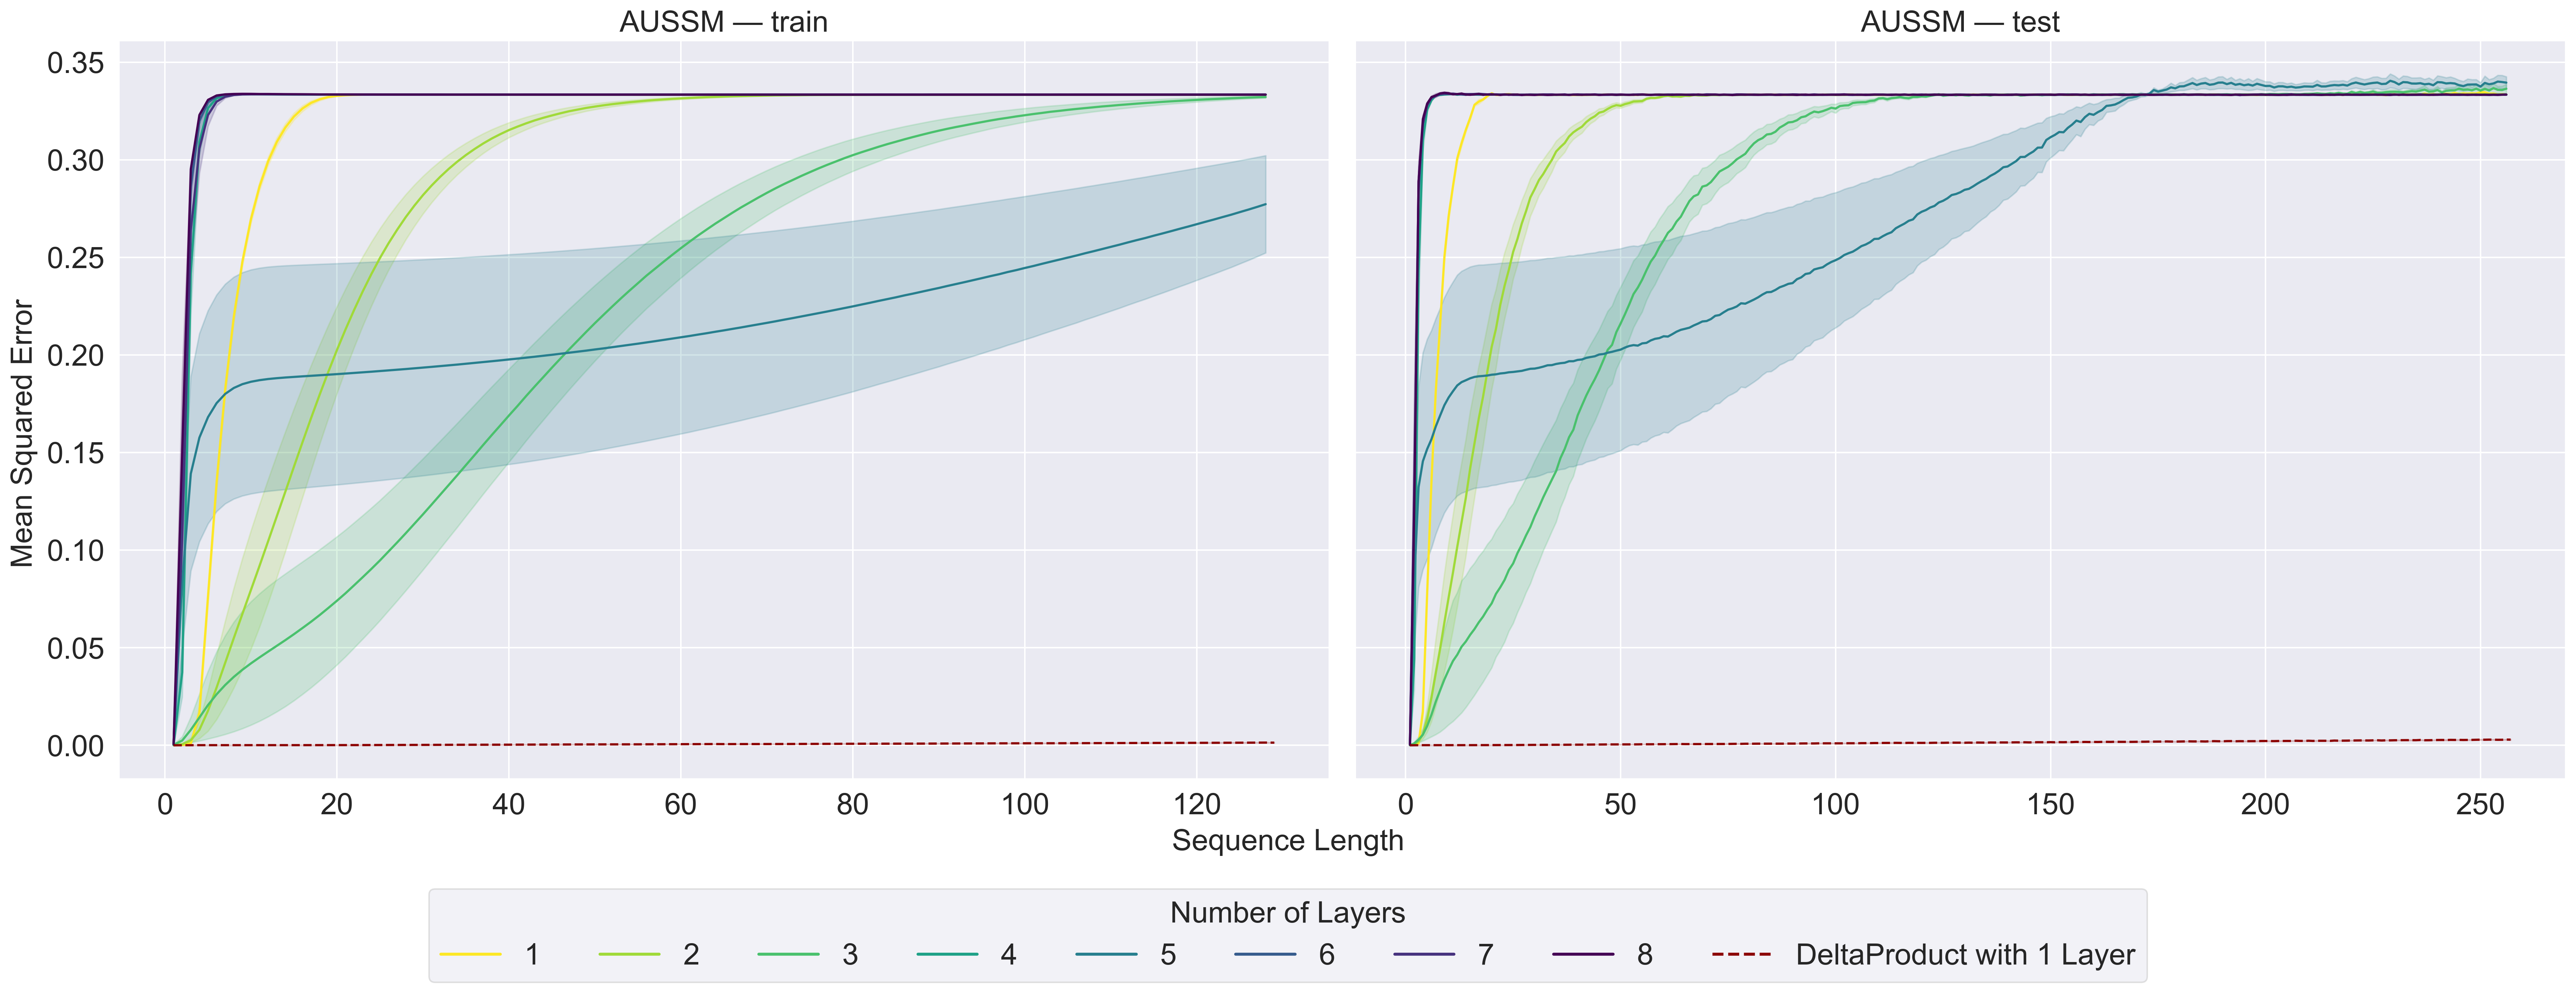
\includegraphics[width=0.95\columnwidth]{figures/mse_grid_aussm.png}
        \caption{Mean squared loss on the rotated vector prediction task at various sequence length for AUSSM, with different numbers of layers, on train (left) and test (right) sets. Standard error is shown using 3 seeds. Performance of DeltaProduct with 4 Householder products is shown as a reference.
}
        \label{fig:rotation_mse_aussm}
    \end{center}
\end{figure*}
